\documentclass[aspectratio=169]{beamer}

\usetheme{Madrid}
\usecolortheme{default}

\usepackage{amsmath, amssymb, amsfonts, mathtools}
\usepackage{bm}
\usepackage{tikz}
\usetikzlibrary{arrows.meta, positioning}

\title{Existence of Solutions for a Stationary Mean Field Game System}
\author{Avi Wine}
\date{March 2026}

\newcommand{\Om}{\Omega}
\newcommand{\Hone}{H_0^1(\Omega)}
\newcommand{\Ltwo}{L^2(\Omega)}

\begin{document}

%------------------------------------------------
\begin{frame}
  \titlepage
\end{frame}

%------------------------------------------------
\begin{frame}{Mean Field Games}
\begin{itemize}
    \item Mean field games model systems with a \textbf{very large number of agents}.
    \item Each individual agent has \textbf{negligible influence} on the overall system.
    \item The discrete population is replaced by a \textbf{continuum density}.
    \item Agents react to the \textbf{aggregate behaviour} of the population.
\end{itemize}

\vspace{0.4cm}

Typical examples include:
\begin{itemize}
    \item financial markets,
    \item crowd motion,
    \item traffic flow.
\end{itemize}
\end{frame}

%------------------------------------------------
\begin{frame}{The Stationary Mean Field Game System}
We study the coupled PDE system
\begin{block}{Stationary Mean Field Game System}
\[
-\Delta u + H(x,\nabla u) + \lambda u = f(x,m)
\qquad \text{in } \Omega \qquad \text{(HJB)}
\]

\[
-\Delta m - \operatorname{div}\!\left(m \frac{\partial H}{\partial p}(x,\nabla u)\right) + \lambda m = G(x)
\qquad \text{in } \Omega \qquad \text{(KFP)}
\]
\end{block}
with homogeneous Dirichlet boundary conditions
\[
u = 0, \qquad m = 0 \qquad \text{on } \partial \Omega.
\]

\vspace{0.3cm}

\begin{itemize}
    \item \(u(x)\): value function of a representative agent
    \item \(m(x)\): density of players
\end{itemize}
\end{frame}

%------------------------------------------------
\begin{frame}{The Coupling Mechanism}
\centering
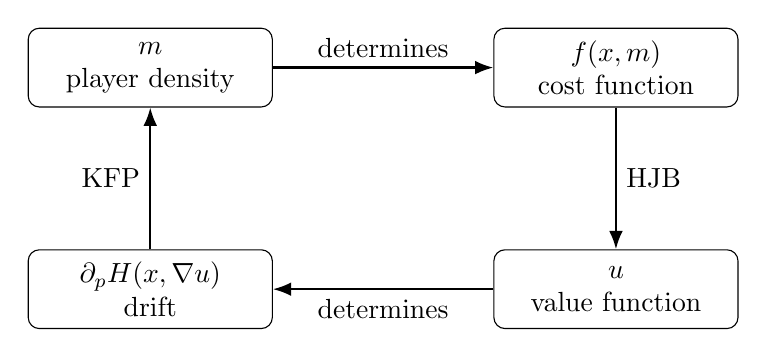
\begin{tikzpicture}[
    node distance=1.8cm and 2.8cm,
    every node/.style={align=center},
    box/.style={draw, rounded corners, minimum width=3.1cm, minimum height=1cm},
    >=Latex
]
\node[box] (m) {\(m\)\\player density};
\node[box, right=of m] (f) {\(f(x,m)\)\\cost function};
\node[box, below=of f] (u) {\(u\)\\value function};
\node[box, below=of m] (drift) {\(\partial_p H(x,\nabla u)\)\\ drift};

\draw[->, thick] (m) -- node[above] {determines} (f);
\draw[->, thick] (f) -- node[right] {HJB} (u);
\draw[->, thick] (u) -- node[below] {determines} (drift);
\draw[->, thick] (drift) -- node[left] {KFP} (m);
\end{tikzpicture}

\vspace{0.5cm}

A solution pair \((u,m)\) represents a \textbf{self-consistent equilibrium}.
\end{frame}

%------------------------------------------------
\begin{frame}{Main Result}
\begin{block}{Theorem}
Under suitable assumptions on \(H\), \(f\), \(G\), the domain \(\Omega\), and for \(\lambda > 0\) sufficiently large, there exists a solution pair
\[
(u,m) \in H_0^1(\Omega)\times H_0^1(\Omega)
\]
to the stationary mean field game system.
\end{block}

\vspace{0.4cm}

\begin{itemize}
    \item \(u\) gives the optimal strategy of a representative agent.
    \item \(m\) gives the resulting equilibrium distribution of agents.
    \item Existence of such a pair corresponds to a Nash equilibrium in the mean field game.
\end{itemize}
\end{frame}

%------------------------------------------------
\begin{frame}{Strategy of the Proof}
The proof has \textbf{two stages}:

\vspace{0.2cm}

\begin{enumerate}
    \item Solve each equation \textbf{independently}:
    \begin{itemize}
        \item HJB for fixed \(m\),
        \item KFP for fixed \(u\).
    \end{itemize}

    \item Combine the resulting solution operators via a \textbf{fixed point argument}.
\end{enumerate}

\vspace{0.5cm}

Define
\[
T[m] = u, \qquad S[u] = m,
\]
and then
\[
A := S\circ T.
\]

If \(A\) has a fixed point, then the coupled system has a solution pair.
\end{frame}

%------------------------------------------------
\begin{frame}{Fixed Point Interpretation}

\centering

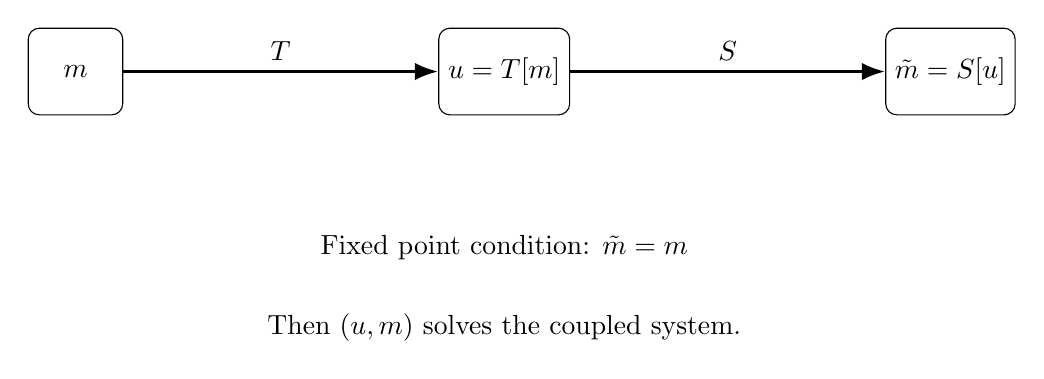
\begin{tikzpicture}[
    node distance=4cm,
    box/.style={draw, rounded corners, minimum width=1.2cm, minimum height=1.1cm, align=center},
    >=Latex
]

\node[box] (m) {$m$};

\node[box, right=of m] (u) {$u = T[m]$};

\node[box, right=of u] (mt) {$\tilde m = S[u]$};

\draw[->, very thick] (m) -- (u)
    node[midway, above, fill=none, draw=none] {$T$};

\draw[->, very thick] (u) -- (mt)
    node[midway, above, fill=none, draw=none] {$S$};


\node[below=1.4cm of u, draw=none] {Fixed point condition: $\tilde{m} = m$};

\node[below=2.4cm of u, draw=none] {Then $(u,m)$ solves the coupled system.};

\end{tikzpicture}

\end{frame}
%------------------------------------------------
\begin{frame}{Step 1: Solving KFP for Fixed \(u\)}
For fixed \(u\), the equation
\[
-\Delta m - \operatorname{div}\!\left(m \frac{\partial H}{\partial p}(x,\nabla u)\right) + \lambda m = G(x)
\]
is \textbf{linear in \(m\)}.

\vspace{0.3cm}

We write the weak formulation
\[
a(m,v)=\ell(v)
\]
with
\[
a(m,v)=\int_\Omega \nabla m\cdot \nabla v
+ m\, \nabla v \cdot \frac{\partial H}{\partial p}(x,\nabla u)
+ \lambda mv \, dx
\]
and
\[
\ell(v)=\int_\Omega G(x)v\,dx.
\]

\vspace{0.3cm}

Then apply the \textbf{Lax--Milgram theorem}.
\end{frame}

%------------------------------------------------
\begin{frame}{Why Lax--Milgram Applies}
To use Lax--Milgram, we show:
\begin{itemize}
    \item \textbf{Boundedness} of the bilinear form \(a(\cdot,\cdot)\),
    \item \textbf{Coercivity} of \(a(\cdot,\cdot)\) for \(\lambda\) sufficiently large.
\end{itemize}

\vspace{0.4cm}

A key estimate is
\[
a(v,v)\ge
\left(1-\frac{\varepsilon^2}{2}\right)\|\nabla v\|_{L^2}^2
+
\left(\lambda-\frac{L^2}{2\varepsilon^2}\right)\|v\|_{L^2}^2.
\]

Hence \(a\) is coercive if \(\lambda\) is sufficiently large.
\end{frame}

%------------------------------------------------
\begin{frame}{Conclusion for KFP}
\begin{block}{Main Result}
For every fixed \(u\in H_0^1(\Omega)\), there exists a \textbf{unique}
\[
m\in H_0^1(\Omega)
\]
solving the KFP equation.
\end{block}

\vspace{0.4cm}

So we obtain a well-defined operator
\[
S : H_0^1(\Omega)\to H_0^1(\Omega), \qquad S[u]=m.
\]

An important result of using Lax-Milgram is that image of \(S\) is bounded. 
\end{frame}
%------------------------------------------------
\begin{frame}{Step 2: Solving HJB for Fixed \(m\)}
For fixed \(m\), the equation
\[
-\Delta u + H(x,\nabla u) + \lambda u = f(x,m)
\]
is \textbf{nonlinear in \(u\)}.

\vspace{0.4cm}

So Lax--Milgram does not apply directly.

\vspace{0.4cm}

Instead, define a map
\[
A[u]=w
\]
where \(w\)  solves

\[\int_\Omega \nabla w \cdot \nabla v + \lambda w \cdot v \,dx = \int_\Omega (f(x,m) - H(x,\nabla u))\cdot v \,dx, \text{ for any } v \in H^1_0(\Omega)\]

A fixed point of this map gives a solution of HJB.
\end{frame}

%------------------------------------------------
\begin{frame}{Schaefer's Fixed Point Theorem}

\begin{block}{Schaefer's Theorem}
Let \(X\) be a Banach space and \(A:X\to X\) a continuous compact map.

If the set
\[
\{u\in X : u = \mu A[u] \text{ for some } \mu\in[0,1]\}
\]
is bounded, then \(A\) has a fixed point.
\end{block}

\vspace{0.4cm}

To apply this result to the HJB equation, we verify:
\begin{itemize}
\item continuity of the operator,
\item compactness,
\item boundedness of the Schaefer set.
\end{itemize}

\end{frame}
%------------------------------------------------
\begin{frame}{Conclusion for HJB}
Using Schaefer's theorem, we obtain existence of a solution \(u\).

\vspace{0.3cm}

Under the largeness assumption on \(\lambda\), uniqueness also follows from an energy estimate.

\vspace{0.4cm}

\begin{block}{Result}
For every fixed \(m\in H_0^1(\Omega)\), there exists a unique
\[
u\in H_0^1(\Omega)
\]
solving the HJB equation.
\end{block}

\vspace{0.4cm}

Hence we obtain a second operator
\[
T : H_0^1(\Omega)\to H_0^1(\Omega), \qquad T[m]=u.
\]
\end{frame}

%------------------------------------------------
\begin{frame}{Solving the Coupled System}
Now combine the two solution operators:
\[
T[m]=u,\qquad S[u]=m,\qquad A=S\circ T.
\]

Again we apply \textbf{Schaefer's theorem}, so we need to show:\\
\textbf{Continuity, Compactness and Boundedness.}

\vspace{0.4cm}

\textbf{Compactness}
\begin{itemize}
    \item Solutions of the HJB equation satisfy an \(H^2\)-bound,
    \item bounded sequences in \(H^2(\Omega)\cap H_0^1(\Omega)\) are precompact in \(H_0^1(\Omega)\),
    \item  therefore \(T\) is compact, and hence \(A=S\circ T\) is compact.
\end{itemize}
\end{frame}
%------------------------------------------------
\begin{frame}{Main Existence Result}
\begin{block}{Conclusion}
The map
\[
A=S\circ T
\]
has a fixed point.
\end{block}

Therefore there exists
\[
(u,m)\in H_0^1(\Omega)\times H_0^1(\Omega)
\]
solving the stationary mean field game system.
\end{frame}

%------------------------------------------------
\begin{frame}{Extension to Nonlinear KFP}
The project also considers the extension
\[
-\Delta m - \operatorname{div}\!\left(m \frac{\partial H}{\partial p}(x,\nabla u)\right) + \lambda m = G(x,m).
\]

\vspace{0.4cm}

Here \(G\) is assumed to be:
\begin{itemize}
    \item Lipschitz continuous in \(m\),
    \item bounded by \(B(|m| + 1)\) for some \(B >0\).
\end{itemize}

\vspace{0.4cm}

The same fixed point framework can be adapted to this setting.
\end{frame}

%------------------------------------------------
\begin{frame}{Result for the Nonlinear KFP Extension}
With suitable assumptions on \(G(x,m)\) and \(\lambda\) sufficiently large:
\begin{itemize}
    \item the nonlinear KFP equation can be solved for fixed \(u\),
    \item the associated operator remains continuous and bounded,
    \item Schaefer's theorem again yields a fixed point.
\end{itemize}

\vspace{0.4cm}

\begin{block}{Extended result}
The mean field game system with nonlinear source term \(G(x,m)\) also admits a solution
\[
(u,m)\in H_0^1(\Omega)\times H_0^1(\Omega).
\]
\end{block}
\end{frame}

%------------------------------------------------
\begin{frame}{Conclusion}
\begin{itemize}
    \item We studied a stationary mean field game system coupling HJB and KFP.
    \item Each equation was first solved independently.
    \item The coupled system was then solved via a fixed point argument.
    \item The main tools were:
    \begin{itemize}
        \item Lax--Milgram,
        \item Schaefer's fixed point theorem,
        \item Rellich--Kondrachov compactness.
    \end{itemize}
    \item The argument extends to a nonlinear source term in the KFP equation.
\end{itemize}
\end{frame}

\end{document}